\documentclass{/home/janmebows/Documents/LatexTemplates/myassignment}
\title{Topic C Assignment 3}

\begin{document}

\maketitle
\begin{enumerate}
	\item \begin{enumerate}
		\item 
		\begin{align*}
			\epsilon \frac{d^2y}{dx^2} + (\cosh x) \frac{dy}{dx} - y= 0\\
		\end{align*}
		To leading order:
		\[y = y_0 + \bigo(\epsilon)\]
		\begin{align*}
			(\cosh x)\frac{dy_0}{dx} - y_0 = 0\\
			\frac{1}{y_0}\frac{dy_0}{dx} = \frac{1}{\cosh x} 
		\end{align*}
		Let $x = x_* + \delta_1 X$, and $y = \delta_2 Y$
		\begin{align*}
			\epsilon \frac{\delta_2^2}{\delta_1^2}\frac{d^2Y}{dX^2} + (\cosh(x_* + \delta_1 X))\frac{\delta_2}{\delta_1} \frac{dY}{dX} - \delta_2 Y= 0\\
		\end{align*}
		With BCs $\delta_2 Y(0) = \delta_2 Y(1) = 1$ Hence $\delta_2 = 1$.
		\[\epsilon \frac{1}{\delta_1}\frac{d^2Y}{dX^2} + (\cosh(x_* + \delta_1 X))\frac1{\delta_1} \frac{dY}{dX} - Y= 0\]
		Expand the $\cosh$ term:
		\begin{align*}
			\cosh (x_*+\delta_1 X) &= \cosh(x_*)\cosh(\delta_1X) + \sinh(x_*)\sinh(\delta_1X)\\
			&=\sinh(x_*)\sum_{i=0}^\infty \frac{(\delta_1 X)^{2i+1}}{(2i+1)!}   + \cosh(x_*)\sum_{i=0}^\infty \frac{(\delta_1 X)^{2i}}{(2i)!}\\
			&= \sinh(x_*)\left(\delta_1 X\right) + \cosh(x_*) + \bigo(\epsilon^2) 
		\end{align*}
		\[\epsilon \frac{1}{\delta_1}\frac{d^2Y}{dX^2} + (\sinh(x_*)\left(\delta_1 X\right) + \cosh(x_*))\frac1{\delta_1} \frac{dY}{dX} - Y= 0\]
		% \[\cosh(x+\delta_1X) =\sum_{i=0}^\infty \frac{(x+\delta_1 X)^{2i}}{(2i)!} = 1 + \frac{(x+\delta_1X)^2}{2} \]
		Possible balances:
		\begin{itemize}
			\item 
			\[\]
		\end{itemize}

		\begin{align*}
			y_{comp} &= y_{in} + y_{out} - y_{overlap}\\
			&=
		\end{align*}
		\item 
		\item First rewrite the BVP in a nicer format
		\[\frac{d^2y}{dx^2} + \frac{1}{\epsilon} \left(\cosh x\frac{dy}{dx} - y\right) = 0\] 
		Figure~\ref{fig:q1}
	\begin{figure}[tb]
		\centering
		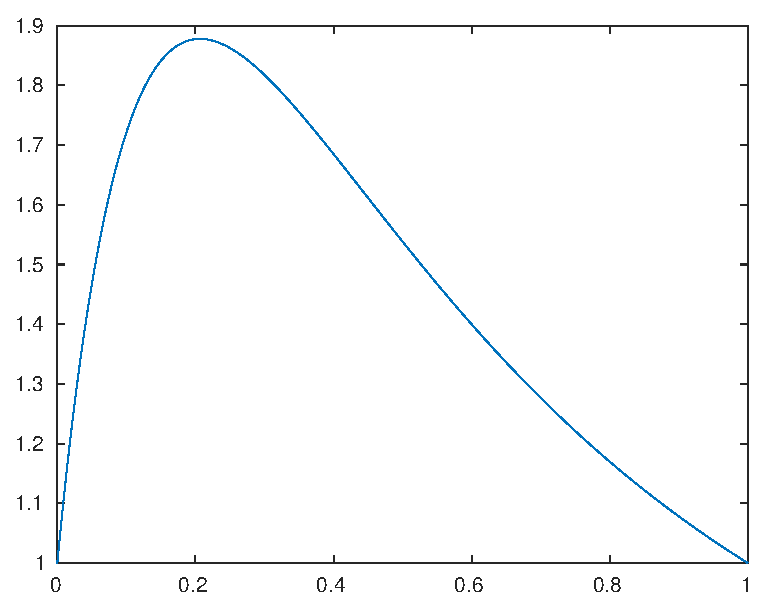
\includegraphics{TopicCA3Q1}
		\caption{Comparison of Numerical, WKB and Composite solutions}
		\label{fig:q1}
	\end{figure}
	\end{enumerate}



	\[\epsilon\frac{\mathrm{d}^2y}{\mathrm{d}x^2}+(2x+1)\frac{\mathrm{d}y}{\mathrm{d}x}+2y=0\]
	\item 
	%Find leading order solutions to
	\[\epsilon \frac{d^2y}{dx^2} + x\frac{dy}{dx} + xy =0\]
	With $y(-2)=-4$ and $y(2) =2$, $\epsilon \to 0$ over $-2\leq x \leq 2$. There is an internal boundary layer shown via the numerical solution, in figure~\ref{fig:q2}

	The right outer solution $y_R$ with $y_R(2) = 2$ to leading order:
	\begin{align*}
	xy_{R0}' + xy_{R0} = 0\\
	y_{R0}' + y_{R0} = 0\\
	y_{R0} = Ae^{-x}
	\end{align*}
	And applying the boundary condition:
	\begin{align*}
		y_{R0}(2) = Ae^{-2} = 2\\
		A = 2e^2
	\end{align*}

	
	The left outer solution $y_L$ with $y_L(-2) =-4$
	\begin{align*}
	y_{L0} = Be^{-x}\\
	y_{L0}(-2) = Be^{-2} = -4\\
	B = -4e^{-2}
	\end{align*}

	For the inner solution $x = x_* + \delta_1 X$, and $y = \delta_2 Y$. Since the boundary conditions don't include $\epsilon$, $\delta_2 =1$.
	\begin{align*}
		\epsilon \frac{d^2y}{dx^2} + x\frac{dy}{dx} + xy =0\\
		\epsilon \frac{1}{\delta_1^2}\frac{d^2Y}{dX^2} + (x^* + \delta_1X)\frac{1}{\delta_1}\frac{dY}{dX} + (x^* +\delta_1 X)Y =0\\
		\epsilon \frac{d^2Y}{dX^2} + \delta_1 (x^* + \delta_1 X)\frac{dY}{dX} + \delta_1^2 (x^* + \delta_1X)Y = 0
	\end{align*}
	
	%%%%ALl this is wrong
	% Balances:
	% \begin{itemize}
	% 	\item $\epsilon \frac{d^2Y}{dX^2} \sim - \delta_1^2 X\frac{dY}{dX}$, neglect $\delta_1^3 XY$, giving $\delta_1 = \sqrt{\epsilon}$, and since $\delta_1^3 = \epsilon^{3/2} \ll \epsilon = \delta_1^2$, this is reasonable.
	% 	\item $\epsilon \frac{d^2Y}{dX^2} \sim - \delta_1^3 XY$, neglect $\delta_1^2 X\frac{dY}{dX}$. This gives $\delta_1 = \epsilon^{1/3}$, and $\delta_1^3 = \epsilon \gg \epsilon^{2/3} =\delta_1^2$, which is a contradiction.
	% 	\item $\delta_1^2 X\frac{dY}{dX} \sim - \delta_1^3 XY = 0$, neglect $\epsilon \frac{d^2Y}{dX^2}$ This gives $\delta_1 =1$, which is the outer solution we have already solved.

	% \end{itemize}
	% Hence $\delta_1 = \sqrt{\epsilon}$

	% So $x = x_* + \epsilon^{1/2}X$. Take the expansion $Y(X) = Y_0 + \epsilon^{1/2} Y_1 + \hdots$.

	% To leading order:
	% \begin{align*}
	% \frac{d^2Y_0}{dX^2} + X\frac{dY_0}{dX} = 0\\
	% \frac{V'}{V} =-X\\
	% V = e^{-X}
	% \end{align*}

	\begin{figure}[tb]
		\centering
		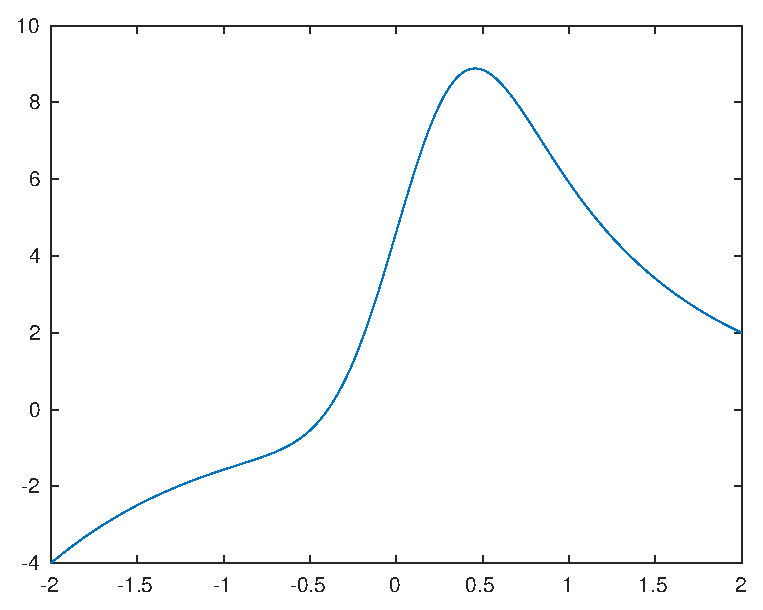
\includegraphics{TopicCA3Q2}
		\caption{Caption here}
		\label{fig:q2}
	\end{figure}
\end{enumerate}
\section*{Matlab Code}
\lstinputlisting{AppTopicCA3.m}

\clearpage
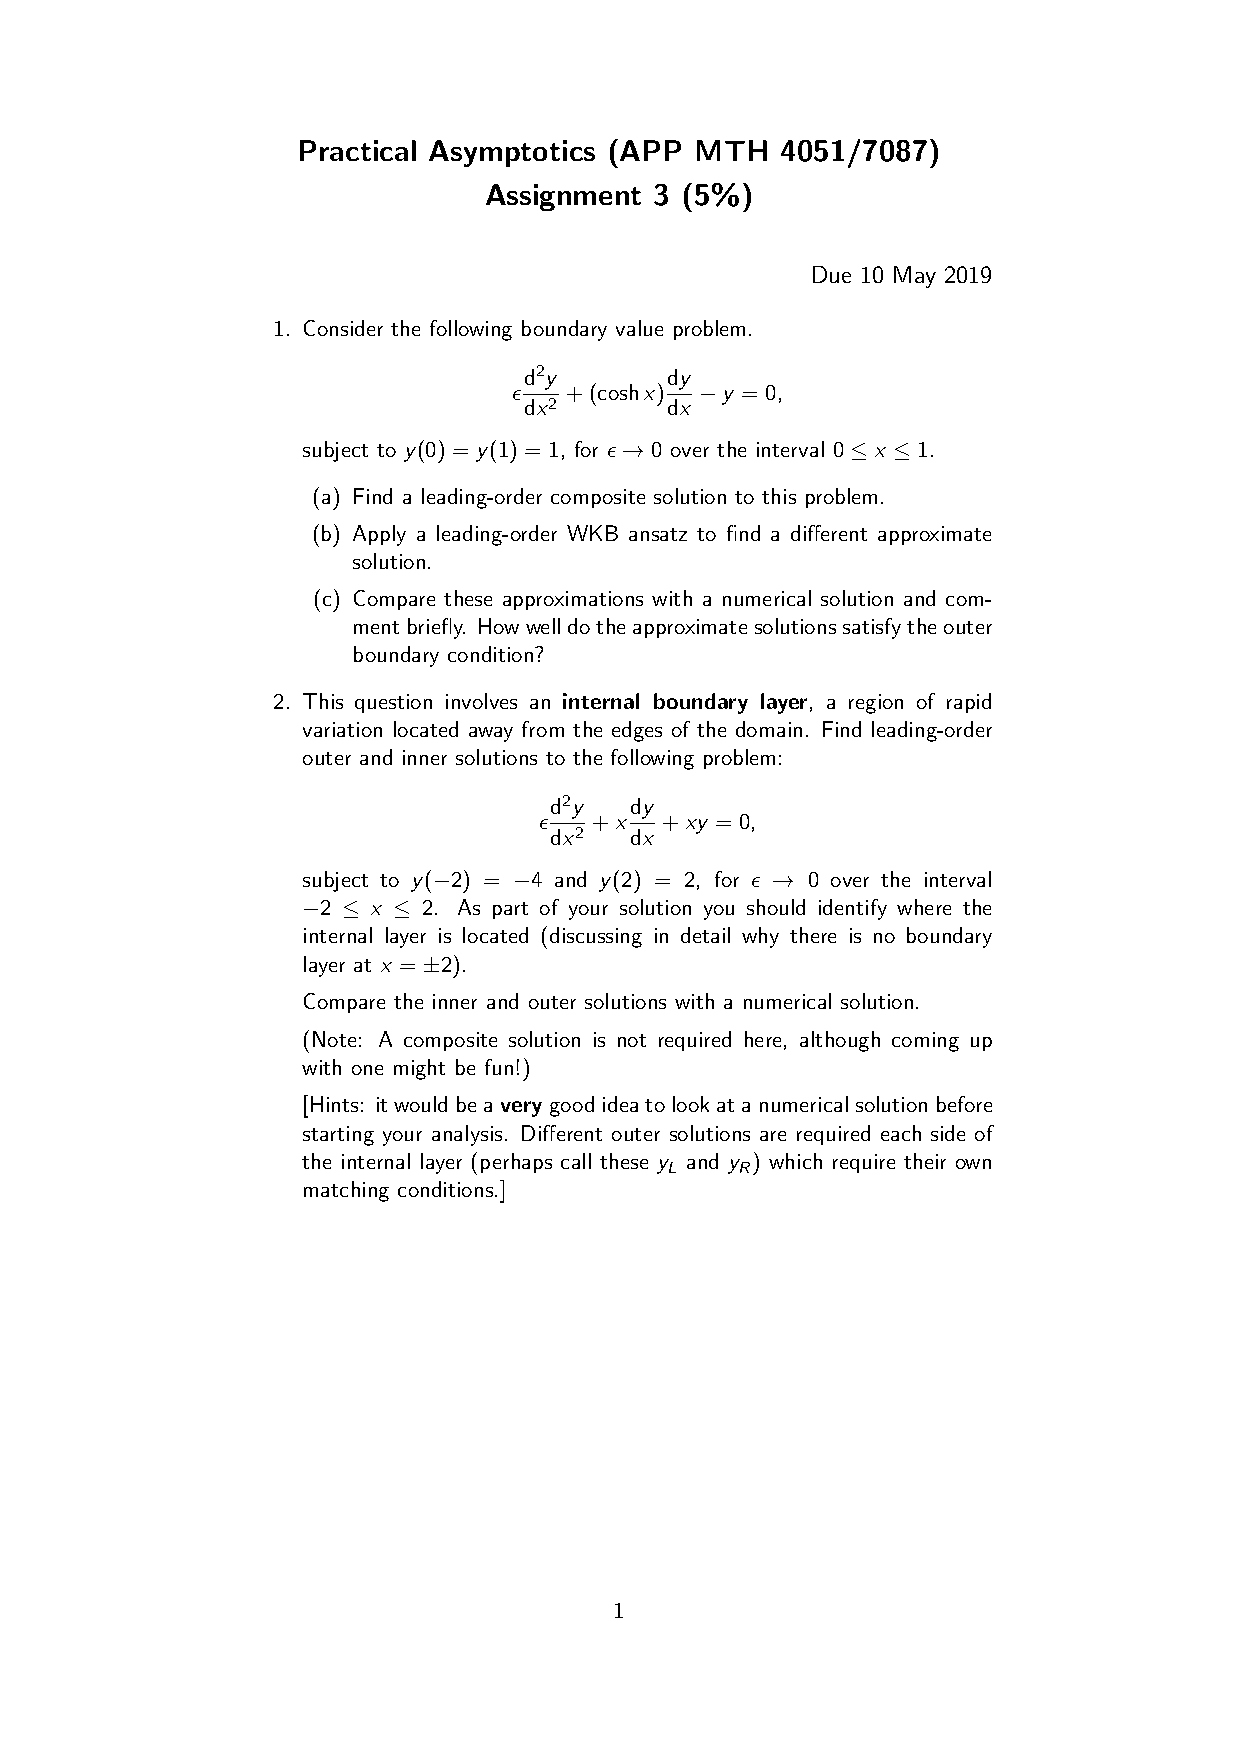
\includepdf[pages=1-]{PA_2019_A3.pdf}

\end{document}